\documentclass[crop,tikz]{standalone}
\usetikzlibrary{backgrounds}
\colorlet{blue}{cyan}
\tikzset{
  inverted/.style = {
    color=white,
    background rectangle/.style={fill},
    show background rectangle
  }
}

\usepackage{tikz-3dplot}

\tikzset{>=latex}

\begin{document}
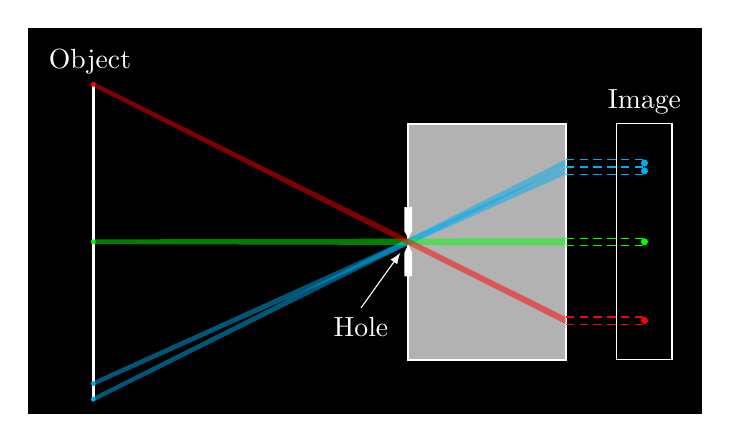
\begin{tikzpicture}[inverted,inverted]
  \pgfmathsetmacro{\xobj}{-4}         % x position of object
  \pgfmathsetmacro{\hobj}{4}          % height of object
  \pgfmathsetmacro{\ximg}{2}          % x position of image
  \pgfmathsetmacro{\himg}{3}          % height of image
  \pgfmathsetmacro{\ximgp}{3}         % x position of projected image
  \pgfmathsetmacro{\rhole}{0.04}      % radius of pinhole
  \pgfmathsetmacro{\robj}{0.03}       % radius of object points
  \pgfmathsetmacro{\rimg}{(\rhole-\robj)/(0-\xobj)*\ximg + \rhole} % radius of image points
  \pgfmathsetmacro{\wimgp}{0.7}       % width of projected image
  % object
  \draw[very thick] ({\xobj},{-\hobj/2}) -- ++ (0,{\hobj}) node[above right,xshift=-2em] {Object};
  % box
  \fill[gray!60] (0,{-\himg/2}) rectangle ({\ximg},{\himg/2});
  \draw[thick] (0,{-\rhole}) -- (0,{-\himg/2}) -- ({\ximg},{-\himg/2}) -- ({\ximg},{\himg/2}) -- (0,{\himg/2}) -- (0,{\rhole});
  \fill (0,{+\rhole}) -- ++ (0.05,+0.1) -- ++ (0,+0.3) -- ++ (-0.1,0) -- ++ (0,-0.3) -- cycle;
  \fill (0,{-\rhole}) -- ++ (0.05,-0.1) -- ++ (0,-0.3) -- ++ (-0.1,0) -- ++ (0,+0.3) -- cycle;
  % projected image
  \draw ({\ximgp-\wimgp/2},{-\himg/2}) rectangle ++ ({\wimgp},{\himg});
  % object coordinates
  \coordinate (OA) at ({\xobj},{-\hobj/2});
  \coordinate (OB) at ({\xobj},{-\hobj*0.45});
  \coordinate (OC) at ({\xobj},0);
  \coordinate (OD) at ({\xobj},{\hobj/2});
  % image coordinates
  \coordinate (IA) at ($\ximg/\xobj*(OA)$);
  \coordinate (IB) at ($\ximg/\xobj*(OB)$);
  \coordinate (IC) at ($\ximg/\xobj*(OC)$);
  \coordinate (ID) at ($\ximg/\xobj*(OD)$);
  % image coordinates of projection
  \coordinate (IAP) at ($(IA)+(\ximgp-\ximg,0)$);
  \coordinate (IBP) at ($(IB)+(\ximgp-\ximg,0)$);
  \coordinate (ICP) at ($(IC)+(\ximgp-\ximg,0)$);
  \coordinate (IDP) at ($(ID)+(\ximgp-\ximg,0)$);
  % help lines
  \draw[blue ,densely dashed] ($(IA)-(0,{\rimg})$) -- ++ ({\ximgp-\ximg},0);
  \draw[blue ,densely dashed] ($(IA)+(0,{\rimg})$) -- ++ ({\ximgp-\ximg},0);
  \draw[cyan ,densely dashed] ($(IB)-(0,{\rimg})$) -- ++ ({\ximgp-\ximg},0);
  \draw[cyan ,densely dashed] ($(IB)+(0,{\rimg})$) -- ++ ({\ximgp-\ximg},0);
  \draw[green,densely dashed] ($(IC)-(0,{\rimg})$) -- ++ ({\ximgp-\ximg},0);
  \draw[green,densely dashed] ($(IC)+(0,{\rimg})$) -- ++ ({\ximgp-\ximg},0);
  \draw[red  ,densely dashed] ($(ID)-(0,{\rimg})$) -- ++ ({\ximgp-\ximg},0);
  \draw[red  ,densely dashed] ($(ID)+(0,{\rimg})$) -- ++ ({\ximgp-\ximg},0);
  % object points
  \fill[blue]  (OA) circle ({\robj});
  \fill[cyan]  (OB) circle ({\robj});
  \fill[green] (OC) circle ({\robj});
  \fill[red]   (OD) circle ({\robj});
  % image points of projection
  \fill[blue]  (IAP) circle ({\rimg});
  \fill[cyan]  (IBP) circle ({\rimg});
  \fill[green] (ICP) circle ({\rimg});
  \fill[red]   (IDP) circle ({\rimg});
  % rays
  \fill[blue ,opacity=0.5] ($(OA)+(0,{\robj})$) -- ($(OA)-(0,{\robj})$) -- ($(IA)-(0,{\rimg})$) -- ($(IA)+(0,{\rimg})$);
  \fill[cyan ,opacity=0.5] ($(OB)+(0,{\robj})$) -- ($(OB)-(0,{\robj})$) -- ($(IB)-(0,{\rimg})$) -- ($(IB)+(0,{\rimg})$);
  \fill[green,opacity=0.5] ($(OC)+(0,{\robj})$) -- ($(OC)-(0,{\robj})$) -- ($(IC)-(0,{\rimg})$) -- ($(IC)+(0,{\rimg})$);
  \fill[red  ,opacity=0.5] ($(OD)+(0,{\robj})$) -- ($(OD)-(0,{\robj})$) -- ($(ID)-(0,{\rimg})$) -- ($(ID)+(0,{\rimg})$);
  % labels
  \node[above] at ({\ximgp},{\himg/2}) {Image};
  \draw[<-] (-0.1,{-\rhole-0.1}) -- ++ (-0.5,-0.7) node[below] {Hole};
\end{tikzpicture}
\end{document}
